% !TeX TXS-program:compile = txs:///pdflatex/[--shell-escape]

\documentclass[11pt, letterpaper]{article}

\usepackage[utf8]{inputenc}
\usepackage{minted}
\usepackage[T1]{fontenc}
\usepackage{lmodern}
\usepackage{graphicx}
\usepackage{longtable}
\usepackage{wrapfig}
\usepackage{rotating}
\usepackage{amsmath}
\usepackage{textcomp}
\usepackage{amssymb}
\usepackage{hyperref}
\usepackage[spanish]{babel}
\usepackage[round]{natbib}
\usepackage{subcaption}

\title{\bfseries Tarea}
\author{Ángel García Báez}
\date{\today}
\setcounter{tocdepth}{4} 

\begin{document}
	
	% Página de presentación
	\begin{titlepage}
		\centering
		
\includegraphics[width=0.2\textwidth]{logo.png}\par
		\vspace{1cm}
		{\LARGE \bfseries Universidad Veracruzana \par}
		\vspace{1cm}
		{\Large Maestría en Inteligencia Artificial\par}
		\vspace{3cm}
		{\LARGE \bfseries Lógica difusa \par}
		\vspace{1cm}
		{\Large \bfseries Tarea 6. Problema del mesero con lógica difusa usando el método de Sugeno con FuzzyToolbox y en código matlab. \par}
		\vfill
		{\Large \textit{Ángel García Báez}\par}
		\vfill
		{\Large Dr. Sergio Hernández Méndez \par}
		\vfill
		{\Large \today \par}
	\end{titlepage}
	
	% Página exclusiva para la tabla de contenidos
	\newpage
	\tableofcontents
	\newpage
	
% Explicación breve

\section{Introducción}

En el presente reporte se plantea el problema de la propina que se le sugiere dejar al mesero en base a la calidad de la comida y a la calidad de la atención del servicio con lógica difusa y usando el método de Sugeno. Para ello, se retomo gran parte de este problema que se ah venido trabajando desde la tarea 1, aplicando ciertas modificaciones a las funciones de membresía, cambiando algunas reglas y modificando las salidas. Para ello, se diseño con ayuda del fuzzytoolbox de matlab y posteriormente se hizo la implementación del codigo en matlab. Se muestra la comparativa de los resultados obtenidos tanto con el fuzzy toolbox como con el código hecho en matlab paso a paso para 3 escenarios distintos:

Cuando las 2 condiciones son mínimas, cuando son medias y cuando son máximas.

\newpage


\section{Problema 1: Problema del mesero}

\subsection{Explicación del Problema}

Se tiene el problema de determinar cuanta propina dejarle a un mesero en un restaurante después de comer. Para ello, se toman en cuenta las variables de Servicio y la Comida.

En la tarea 1, se hizo la labor de probar con distintas combinaciones de funciones de membresía y parámetros para suavizar lo más posible la curva. Debido a la implementación del problema con el método de Sugeno, las funciones de membresia de las variables COMIDA y SERVICIO fueron re-hechas como funciones triangulares. Ademas, se agrego otra posible salida al conjunto de la propina, siendo ahora 4 posibles niveles de propina: Nula, baja, media y alta, dichos niveles se modelador como singletons. Finalmente, se modifico la primer regla donde la comida es mala y el servicio es malo para dar como resultado que entonces, la propina es nula.


\subsection{Variables y sus codificaciones}

A continuación se listan los valores de las variables lingüísticas que se propusieron para SERVICIO, COMIDA y PROPINA como sigue:

\begin{enumerate}
	\item Servicio: Malo $[0,0,5]$, Regular $[0.8333,5,9.167]$ y Bueno $[4,10,10]$.
	\begin{figure}[h]
		\centering
		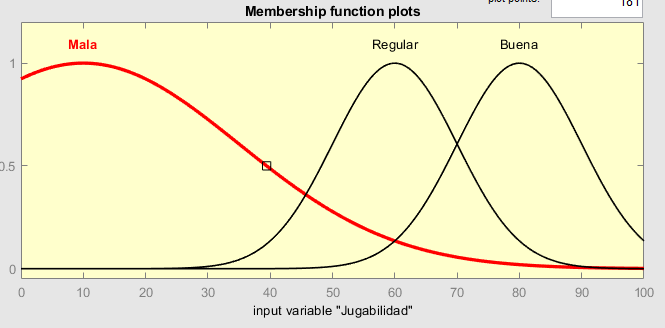
\includegraphics[width=0.8\textwidth]{IMG/P11.png}
		\caption{Funciones de pertenencia triangulares para la variable de entrada Servicio}
	\end{figure}
	
	\newpage
	
	\item Comida: Mala $[0,0,45]$, Normal $[15,45,80]$, Buena $[40,70,95]$ y Excelente $[60,100,100]$.
	\begin{figure}[h]
		\centering
		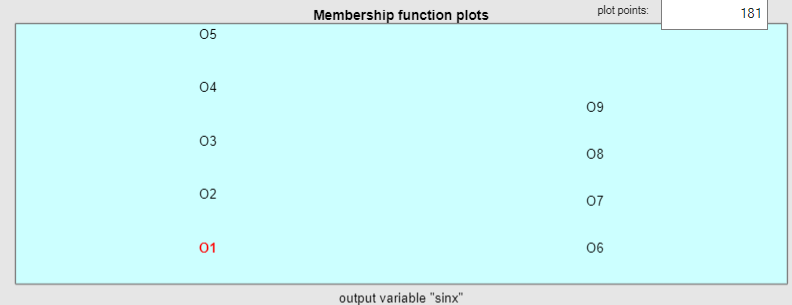
\includegraphics[width=0.8\textwidth]{IMG/P12.png}
		\caption{Funciones de pertenencia triangulares para la variable de entrada Comida}
	\end{figure}
	
	\item Propina: Nula (valor constante de 0), Baja (valor constante de 5), Normal (valor constante de 12) y Alta (valor constante de 20).
	\begin{figure}[h]
		\centering
		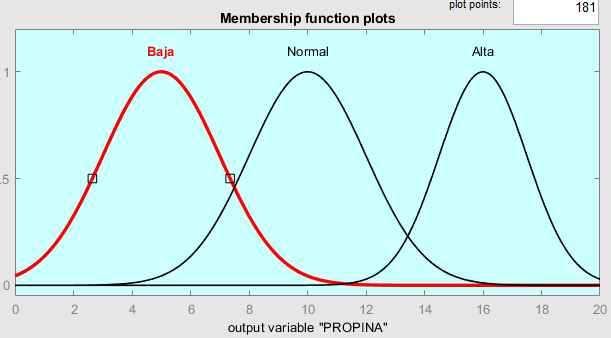
\includegraphics[width=0.8\textwidth]{IMG/P13.png}
		\caption{Valores constantes para la variable de salida Propina (método Sugeno)}
	\end{figure}
\end{enumerate}


Las funciones de membresía de SERVICIO y COMIDA fueron modeladas con triangulares, mientras que la salida de PROPINA fue modelada con singletons (una triangular modificada en 1 solo valor) para mantener el sistema $sencillo$ y por su naturaleza discreta. \\

Se aplico el método de Sugeno para el procesado de las variables de entrada. 

\newpage

\subsection{Reglas de inferencia.}

A continuación se muestran las doce reglas que se construyeron para este problema:

\begin{enumerate}
	\item R1: Si \textbf{SERVICIO} es \textbf{\textit{MALO}} y la \textbf{COMIDA} es \textbf{\textit{MALA}}, la \textbf{PROPINA} es \textbf{\textit{NULA}}.
	\item R2: Si \textbf{SERVICIO} es \textbf{\textit{BUENO}} y la \textbf{COMIDA} es \textbf{\textit{NORMAL}}, la \textbf{PROPINA} es \textbf{\textit{NORMAL}}.
	\item R3: Si \textbf{SERVICIO} es \textbf{\textit{REGULAR}} y la \textbf{COMIDA} es \textbf{\textit{NORMAL}}, la \textbf{PROPINA} es \textbf{\textit{NORMAL}}.
	\item R4: Si \textbf{SERVICIO} es \textbf{\textit{REGULAR}} y la \textbf{COMIDA} es \textbf{\textit{BUENA}}, la \textbf{PROPINA} es \textbf{\textit{NORMAL}}.
	\item R5: Si \textbf{SERVICIO} es \textbf{\textit{BUENO}} y la \textbf{COMIDA} es \textbf{\textit{EXCELENTE}}, la \textbf{PROPINA} es \textbf{\textit{ALTA}}.
	\item R6: Si \textbf{SERVICIO} es \textbf{\textit{MALO}} y la \textbf{COMIDA} es \textbf{\textit{EXCELENTE}}, la \textbf{PROPINA} es \textbf{\textit{BAJA}}.
	\item R7: Si \textbf{SERVICIO} es \textbf{\textit{BUENO}} y la \textbf{COMIDA} es \textbf{\textit{MALA}}, la \textbf{PROPINA} es \textbf{\textit{BAJA}}.
	\item R8: Si \textbf{SERVICIO} es \textbf{\textit{MALO}} y la \textbf{COMIDA} es \textbf{\textit{NORMAL}}, la \textbf{PROPINA} es \textbf{\textit{BAJA}}.
	\item R9: Si \textbf{SERVICIO} es \textbf{\textit{MALO}} y la \textbf{COMIDA} es \textbf{\textit{BUENA}}, la \textbf{PROPINA} es \textbf{\textit{BAJA}}.
	\item R10: Si \textbf{SERVICIO} es \textbf{\textit{BUENO}} y la \textbf{COMIDA} es \textbf{\textit{BUENA}}, la \textbf{PROPINA} es \textbf{\textit{ALTA}}.
	\item R11: Si \textbf{SERVICIO} es \textbf{\textit{REGULAR}} y la \textbf{COMIDA} es \textbf{\textit{MALA}}, la \textbf{PROPINA} es \textbf{\textit{BAJA}}.
	\item R12: Si \textbf{SERVICIO} es \textbf{\textit{REGULAR}} y la \textbf{COMIDA} es \textbf{\textit{EXCELENTE}}, la \textbf{PROPINA} es \textbf{\textit{ALTA}}.
\end{enumerate}

\newpage

\subsection{Gráficos del problema del mesero}

La gráfica de superficie resultante de todo lo descrito previamente, es la siguiente:

\begin{figure}[h]
	\centering
	\begin{subfigure}{0.42\textwidth} % Reducido de 0.45
		\centering
		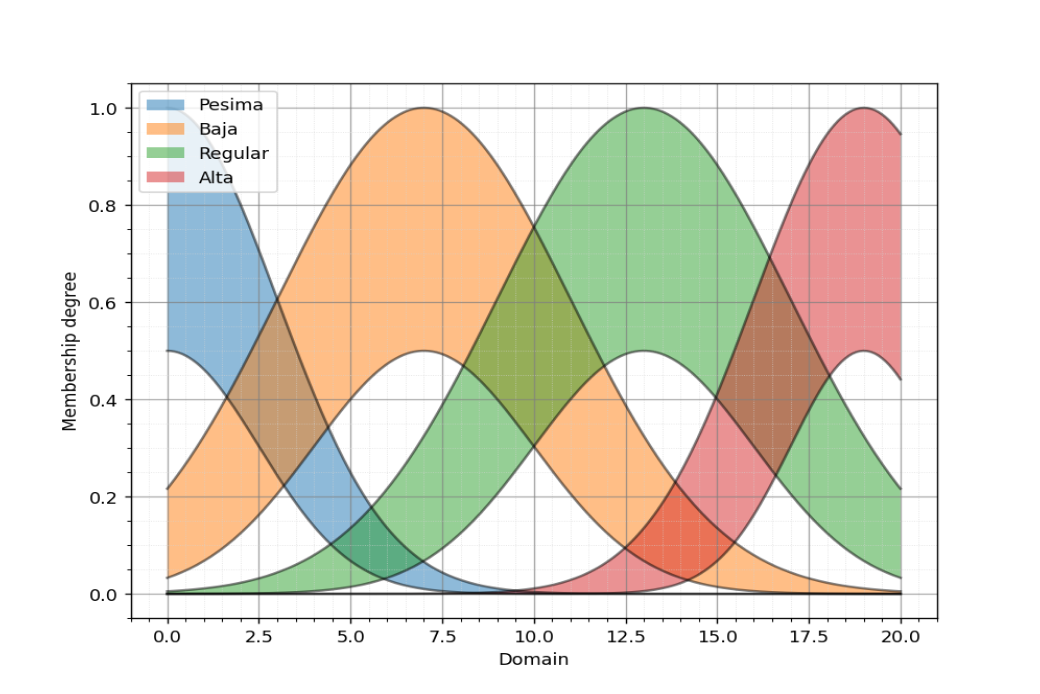
\includegraphics[width=1.3\textwidth]{IMG/P14.png}
		\label{fig:G1}
	\end{subfigure}
	\hfill
	\begin{subfigure}{0.43\textwidth} % Reducido de 0.45
		\centering
		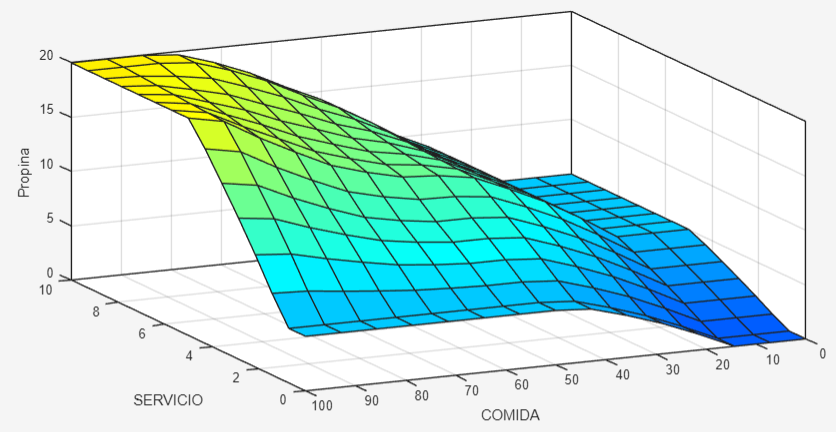
\includegraphics[width=1.2\textwidth]{IMG/P15.png}
		\label{fig:G2}
	\end{subfigure}
	\label{fig:comparacion1}
\end{figure}

La gráfica de superficie muestra un comportamiento suave en el descenso que va teniendo conforme van variando los valores, de aquí cabe señalar 2 cosas: La gráfica logra abarcar todo el rango posible para los valores de la propina y la inclusión de la regla donde la propina es nula produce un cambio drástico que mueve la superficie de golpe hacia 0. 

\newpage

\subsection{Implementación del problema del mesero paso a paso}

Como se menciono en un inicio, el principal objetivo de esta actividad aparte de mostrar los resultados con el método de Sugeno, es implementar uno mismo el sistema de lógica difusa para comparar los resultados con respecto de los mostrados por el fuzzy toolbox de matlab.\\

El primer paso  identificar las variables de discurso SERVICIO, COMIDA y PROPINA para inicializarlas en 0.\\

Con referencia a lo explicado en el libro de \cite{Cisneros2004}, se implemento la función de membresía triangular tal y como la define a continuación:

$$
\mu_A(x) = 
\begin{cases}
	0, & x \le a \\
	\frac{x - a}{b - a}, & a < x \le b \\
	\frac{c - x}{c - b}, & b < x \le c \\
	0, & x > c
\end{cases}
$$


Posteriormente, se definieron los rangos de cada una de las funciones de membresía, dado que solo se usan funciones triangulares y singletons, se dejaron los rangos tal cual se había presentado anteriormente:


\begin{enumerate}
	\item Servicio: Malo $[0,0,5]$, Regular $[0.8333,5,9.167]$ y Bueno $[4,10,10]$.	
	\item Comida: Mala $[0,0,45]$, Normal $[15,45,80]$, Buena $[40,70,95]$ y Excelente $[60,100,100]$.
	\item Propina: Nula (valor constante de 0), Baja (valor constante de 5), Normal (valor constante de 12) y Alta (valor constante de 20).
\end{enumerate}


Siguiendo con el proceso, fueron implementadas cada una las 12 reglas que ya se mostraron previamente y utilizando los resultados de las funciones de membresía como se describe a continuación:

El valor de activación de la regla:

$$
w_i = \mu_{A_i}(x_1) \cdot \mu_{B_i}(x_2)
$$

La contribución de la regla de salida:

$$
contribucion_i = w_i \cdot z_i
$$

Por ultimo, ya que se contaban con las funciones de membresía y el sistema de reglas, dado que se van a trabajar con salidas singleton, la forma de deffuzificar las entradas para generar las salidas es mediante el método del promedio ponderado:


$$
z = \frac{\sum_{i=1}^{N} w_i \cdot z_i}{\sum_{i=1}^{N} w_i}
$$




donde:

\begin{itemize}
	\item \( x_i \) son los valores discretos de la variable de salida.
	\item \( \mu(x_i) \) es el grado de pertenencia de \( x_i \) en la función de pertenencia de la salida difusa.
	\item \( n \) es el número total de puntos discretos en el dominio de salida.
\end{itemize}

Una vez que el sistema esta listo y programado, se procede a hacer la comparativa con el toolbox de matlab.

\newpage

\subsection{Comparativa para el problema del mesero}

A continuación se presentan los resultados que da el sistema programado paso a paso en matlab contra el resultado para el mismo sistema por parte del fuzzy toolbox en 3 escenarios distintos.

\subsubsection{Caso mínimo}

Para el caso mínimo, se propone un $SERVICIO = 0$ y una $COMIDA = 0$ para ver como se comportan ambas versiones ante situaciones tan extremas.

\begin{figure}[h]
	\centering
	\begin{subfigure}{0.40\textwidth} % Reducido de 0.45
		\centering
		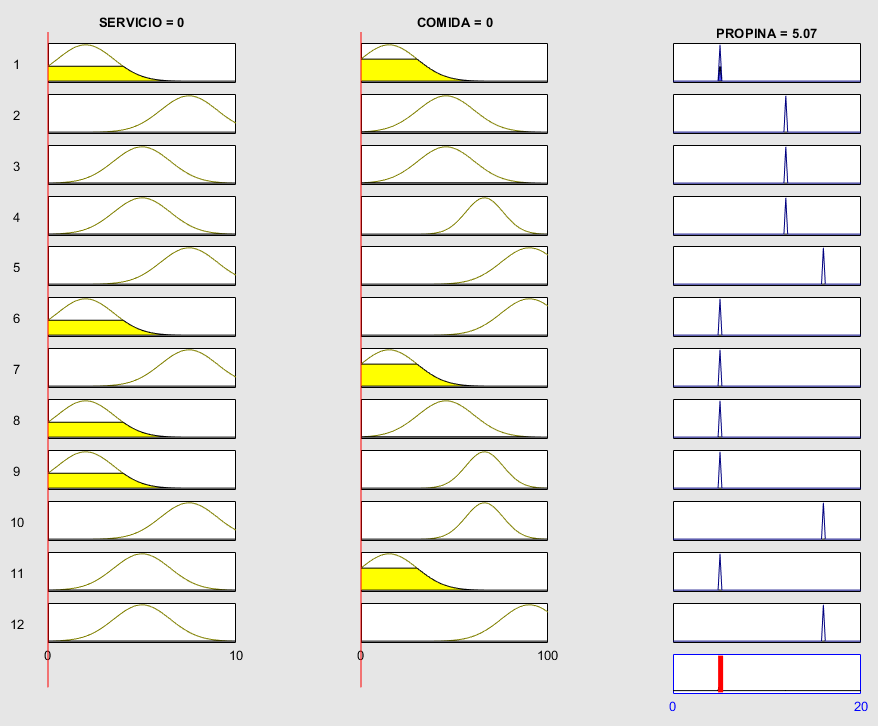
\includegraphics[width=1.4\textwidth]{IMG/RP11.png}
		\label{fig:G3}
	\end{subfigure}
	\hfill
	\begin{subfigure}{0.42\textwidth} % Reducido de 0.45
		\centering
		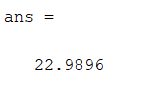
\includegraphics[width=0.4\textwidth]{IMG/M11.png}
		\label{fig:G4}
	\end{subfigure}
	\label{fig:comparacion2}
\end{figure}

A la izquierda se muestran los resultados del toolbox y a la derecha el resultado del sistema programado paso a paso. El toolbox reporta un valor de 0 para el caso planteado, mientras que el sistema programado paso a paso muestra un valor de 0. La diferencia entre ambos casos es nula, por lo que se puede afirmar que llegan al mismo resultado. Un servicio de 0 y una comida de 0 llegan a dar como resultado una propina de 0\% (nula).

\newpage

\subsubsection{Caso medio}
Para el caso medio, se propone un $SERVICIO = 5$ y una $COMIDA = 50$ para ver como se comportan ambas versiones ante situación media.

\begin{figure}[h]
	\centering
	\begin{subfigure}{0.40\textwidth} % Reducido de 0.45
		\centering
		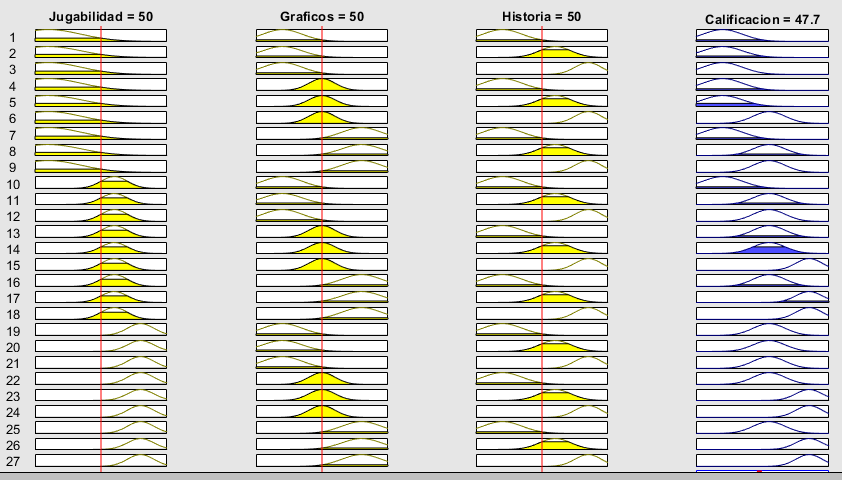
\includegraphics[width=1.4\textwidth]{IMG/RP12.png}
		\label{fig:G5}
	\end{subfigure}
	\hfill
	\begin{subfigure}{0.42\textwidth} % Reducido de 0.45
		\centering
		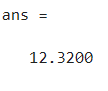
\includegraphics[width=0.4\textwidth]{IMG/M12.png}
		\label{fig:G6}
	\end{subfigure}
	\label{fig:comparacion3}
\end{figure}

A la izquierda se muestran los resultados del toolbox y a la derecha el resultado del sistema programado paso a paso. El toolbox reporta un valor de 12.32 para el caso planteado, mientras que el sistema programado paso a paso muestra un valor de 12.32. La diferencia entre ambos casos es nula, por lo que se puede afirmar que llegan al mismo resultado. Un servicio de 5 y una comida de 50 llegan a dar como resultado una propina de 12.32\% (media).

\newpage

\subsubsection{Caso máximo}
Para el caso máximo, se propone un $SERVICIO = 10$ y una $COMIDA = 100$ para ver como se comportan ambas versiones ante situaciones tan extremas.

\begin{figure}[h]
	\centering
	\begin{subfigure}{0.40\textwidth} % Reducido de 0.45
		\centering
		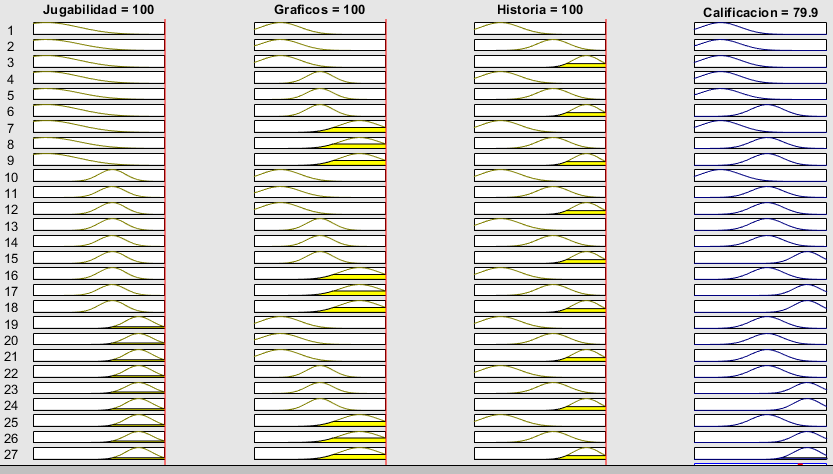
\includegraphics[width=1.4\textwidth]{IMG/RP13.png}
		\label{fig:G7}
	\end{subfigure}
	\hfill
	\begin{subfigure}{0.42\textwidth} % Reducido de 0.45
		\centering
		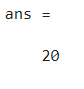
\includegraphics[width=0.4\textwidth]{IMG/M13.png}
		\label{fig:G8}
	\end{subfigure}
	\label{fig:comparacion4}
\end{figure}

A la izquierda se muestran los resultados del toolbox y a la derecha el resultado del sistema programado paso a paso. El toolbox reporta un valor de 20 para el caso planteado, mientras que el sistema programado paso a paso muestra un valor de 20. La diferencia entre ambos casos es nula, por lo que se puede afirmar que llegan al mismo resultado. Un servicio de 20 y una comida de 100 llegan a dar como resultado una propina del 20 \% (Alta).


\section{Conclusiones}

A rasgos generales, los resultados del sistema programado paso a paso y del toolbox de matlab resultan prácticamente iguales en los casos donde se hizo la comparación.

Si bien, no se esta explotando al máximo las bondades del método de Sugeno, como lo es generar salidas a partir de polinomios de grado 1, el método arroja mejores resultados que los encontrados por el método de Mandami de la tarea 2.

\newpage

\section{Referencias}

\bibliographystyle{apalike}  % Estilo de cita, puedes cambiarlo si lo prefieres.
\bibliography{Biblio}         % Aquí incluyes el archivo .bib (sin extensión).

\newpage

\section{Anexos}

Este reporte se envía con los códigos anexos que corresponden a:

\begin{enumerate}
	\item Archivo .fiz del sistema difuso para el problema del mesero con método de Sugeno.
	\item Código en matlab para ejecutar el sistema difuso programado para el problema del mesero con método de Sugeno.

\end{enumerate}



\end{document}

